\documentclass[journal, a4paper]{IEEEtran}

% some very useful LaTeX packages include:
\usepackage{multirow}
\usepackage{listings}
\usepackage[usenames,dvipsnames]{xcolor}
\usepackage{fontspec,xunicode}

\newfontfamily{\monotype}{Fira Code}
\lstset {
  basicstyle = \scriptsize\monotype,
  language = C++,
  tabsize = 2,
  breaklines = true,
  breakindent = 1.1em,
  % numbers=right,
  stringstyle=\monotype,
  numberstyle=\footnotesize\ttfamily,
  firstnumber=last,
  basewidth={0.5em, 0.4em},
}

%\usepackage{cite}      % Written by Donald Arseneau
                        % V1.6 and later of IEEEtran pre-defines the format
                        % of the cite.sty package \cite{} output to follow
                        % that of IEEE. Loading the cite package will
                        % result in citation numbers being automatically
                        % sorted and properly "ranged". i.e.,
                        % [1], [9], [2], [7], [5], [6]
                        % (without using cite.sty)
                        % will become:
                        % [1], [2], [5]--[7], [9] (using cite.sty)
                        % cite.sty's \cite will automatically add leading
                        % space, if needed. Use cite.sty's noadjust option
                        % (cite.sty V3.8 and later) if you want to turn this
                        % off. cite.sty is already installed on most LaTeX
                        % systems. The latest version can be obtained at:
                        % http://www.ctan.org/tex-archive/macros/latex/contrib/supported/cite/

\usepackage{graphicx}   % Written by David Carlisle and Sebastian Rahtz
                        % Required if you want graphics, photos, etc.
                        % graphicx.sty is already installed on most LaTeX
                        % systems. The latest version and documentation can
                        % be obtained at:
                        % http://www.ctan.org/tex-archive/macros/latex/required/graphics/
                        % Another good source of documentation is "Using
                        % Imported Graphics in LaTeX2e" by Keith Reckdahl
                        % which can be found as esplatex.ps and epslatex.pdf
                        % at: http://www.ctan.org/tex-archive/info/

%\usepackage{psfrag}    % Written by Craig Barratt, Michael C. Grant,
                        % and David Carlisle
                        % This package allows you to substitute LaTeX
                        % commands for text in imported EPS graphic files.
                        % In this way, LaTeX symbols can be placed into
                        % graphics that have been generated by other
                        % applications. You must use latex->dvips->ps2pdf
                        % workflow (not direct pdf output from pdflatex) if
                        % you wish to use this capability because it works
                        % via some PostScript tricks. Alternatively, the
                        % graphics could be processed as separate files via
                        % psfrag and dvips, then converted to PDF for
                        % inclusion in the main file which uses pdflatex.
                        % Docs are in "The PSfrag System" by Michael C. Grant
                        % and David Carlisle. There is also some information
                        % about using psfrag in "Using Imported Graphics in
                        % LaTeX2e" by Keith Reckdahl which documents the
                        % graphicx package (see above). The psfrag package
                        % and documentation can be obtained at:
                        % http://www.ctan.org/tex-archive/macros/latex/contrib/supported/psfrag/

%\usepackage{subfigure} % Written by Steven Douglas Cochran
                        % This package makes it easy to put subfigures
                        % in your figures. i.e., "figure 1a and 1b"
                        % Docs are in "Using Imported Graphics in LaTeX2e"
                        % by Keith Reckdahl which also documents the graphicx
                        % package (see above). subfigure.sty is already
                        % installed on most LaTeX systems. The latest version
                        % and documentation can be obtained at:
                        % http://www.ctan.org/tex-archive/macros/latex/contrib/supported/subfigure/

\usepackage{url}        % Written by Donald Arseneau
                        % Provides better support for handling and breaking
                        % URLs. url.sty is already installed on most LaTeX
                        % systems. The latest version can be obtained at:
                        % http://www.ctan.org/tex-archive/macros/latex/contrib/other/misc/
                        % Read the url.sty source comments for usage information.

%\usepackage{stfloats}  % Written by Sigitas Tolusis
                        % Gives LaTeX2e the ability to do double column
                        % floats at the bottom of the page as well as the top.
                        % (e.g., "\begin{figure*}[!b]" is not normally
                        % possible in LaTeX2e). This is an invasive package
                        % which rewrites many portions of the LaTeX2e output
                        % routines. It may not work with other packages that
                        % modify the LaTeX2e output routine and/or with other
                        % versions of LaTeX. The latest version and
                        % documentation can be obtained at:
                        % http://www.ctan.org/tex-archive/macros/latex/contrib/supported/sttools/
                        % Documentation is contained in the stfloats.sty
                        % comments as well as in the presfull.pdf file.
                        % Do not use the stfloats baselinefloat ability as
                        % IEEE does not allow \baselineskip to stretch.
                        % Authors submitting work to the IEEE should note
                        % that IEEE rarely uses double column equations and
                        % that authors should try to avoid such use.
                        % Do not be tempted to use the cuted.sty or
                        % midfloat.sty package (by the same author) as IEEE
                        % does not format its papers in such ways.

\usepackage{amsmath}    % From the American Mathematical Society
                        % A popular package that provides many helpful commands
                        % for dealing with mathematics. Note that the AMSmath
                        % package sets \interdisplaylinepenalty to 10000 thus
                        % preventing page breaks from occurring within multiline
                        % equations. Use:
%\interdisplaylinepenalty=2500
                        % after loading amsmath to restore such page breaks
                        % as IEEEtran.cls normally does. amsmath.sty is already
                        % installed on most LaTeX systems. The latest version
                        % and documentation can be obtained at:
                        % http://www.ctan.org/tex-archive/macros/latex/required/amslatex/math/



% Other popular packages for formatting tables and equations include:

%\usepackage{array}
% Frank Mittelbach's and David Carlisle's array.sty which improves the
% LaTeX2e array and tabular environments to provide better appearances and
% additional user controls. array.sty is already installed on most systems.
% The latest version and documentation can be obtained at:
% http://www.ctan.org/tex-archive/macros/latex/required/tools/

% V1.6 of IEEEtran contains the IEEEeqnarray family of commands that can
% be used to generate multiline equations as well as matrices, tables, etc.

% Also of notable interest:
% Scott Pakin's eqparbox package for creating (automatically sized) equal
% width boxes. Available:
% http://www.ctan.org/tex-archive/macros/latex/contrib/supported/eqparbox/

% *** Do not adjust lengths that control margins, column widths, etc. ***
% *** Do not use packages that alter fonts (such as pslatex).         ***
% There should be no need to do such things with IEEEtran.cls V1.6 and later.


% Your document starts here!
\begin{document}

% Define document title and author
	\title{Gabor Noise Implementation Report}
	\author{Hao Ling - 161180076
	\thanks{}}
	\markboth{NJU Computer Science and Technology, 161180076, Hao Ling}{}
	\maketitle

% Write abstract here
\begin{abstract}
  This is the report for the class assignment about implementating the Gabor Noise.
\end{abstract}

% Each section begins with a \section{title} command
\section{Introduction}
  Gabor noise is a procedural noise generated by Sparse Gabor Convolution and first introduced by
  \cite{lagae2009procedural}. One is able to obtain anisotropic or isotropic Gabor noise of high quality
  within a short evaluating time, and control the appearance of Gabor noise by 
  spectral control. 

% Main Part
\section{Principle}
\subsection{Gabor Kernel}
  The difinition of Gabor Kernel is 

  $$
    g(x, y) = Ke^{-\pi a^2(x^2+y^2)}\cos [ 2\pi F_0 (x\cos \omega_0 + y \sin \omega_0 ) ]
  $$

  The Fourier transform of the Gabor Kernel is
  \begin{gather*}
  \begin{aligned}
    G(f_x, f_y) & = \\ 
    \frac{K}{2a^2} (
    & e^{-\frac{\pi}{a^2} [(f_x - F_0\cos \omega_0)^2) + (f_y - F_0 \sin \omega_0)^2]}+ \\
    & e^{-\frac{\pi}{a^2} [(f_x + F_0\cos \omega_0)^2) + (f_y + F_0 \sin \omega_0)^2]} ) \\
  \end{aligned} 
  \end{gather*}
\subsection{Isotropic Noise with anisotropic kernel}
  With a convolution, we can written down the isotropic Gabor noise generated by the
  anisotropic kernel: 

  $$
    N(x, y) = \sum_{i}w_ig(x - x_i, y - y_i;\omega_{0, i})
  $$

  where $w_{0;i}$ are uniformly sampled from $[0, 2\pi)$, and $x_i, y_i$ are governed by 
  a Poisson distribution with mean $\lambda$. 

\subsection{Anisotropic Noise with anisotropic kernel}
  It is similar with the below one, the only difference is how $w_{0;i}$ are sampled. 
  One can change $[0, 2\pi)$ to any interval $[A, B)$ to control the direction of Gabor noise.

\subsection{Isotropic Noise with isotropic kernel}
  The isotropic Gabor kernel is defined as the product of a a Gaussian and
  a harmonic in spatial domain. 

  With some mathematical deduction, the $n$-dimention Gabor kernel is obtained. 

  $$
    g(r) = Ke^{-\pi a^2 r^2}\frac{2\pi F_0^{\frac{n}{2}}}{r^{\frac{n}{2} - 1}}J_{\frac{n}{2} - 1}(2\pi F_0 r)
  $$

  The $J(x)$ is the order-$n$ Bessel function of first kind.

  I use the code from \cite{press1996numerical} to estimate the value of Bessel function.

\section{Implementation}
  The toolchain used in the experiment is listed below.
  \begin{itemize}
    \item GCC with C++11 support to compile source code. 
    \item opencv2.4 for GUI support.
    \item Mitsuba for rendering.
  \end{itemize}

  \subsection{Interfaces}
  The base class GaborNoise is mainly consist of several important functions listing below. 
  
  \begin{itemize}
    \item get\_fourier(x, y): return the value of kernel's frequency domain at $(x, y)$.
    \item get\_kernel(x, y): return the value of kernel's spatial domain at $(x, y)$.
    \item noise(x, y): return the value of noise at $(x, y)$.
  \end{itemize}

  \begin{lstlisting}[language=C++, caption={GaborNoise Interfaces}]
    class GaborNoise {
    private:
      virtual float_type gabor(
                          float_type K, float_type a, float_type F_0,
                          float_type omega_0, float_type x,
                          float_type y) const;
      virtual float_type fourier(float_type x, float_type y) const;
    public:
      float_type get_fourier(float_type x, float_type y) const;
      float_type get_kernel(float_type x, float_type y) const;
      float_type noise(float_type x, float_type y);
    }
  \end{lstlisting}

  There are also three derived classes overriding the virtual functions \textbf{gabor} and \textbf{fourier}. 
  
  \begin{itemize}
    \item GaborNoise\_anisotropic: producing anisotropic noise with anisotropic kernel.
    \item GaborNoise\_isotropic: producing isotropic noise with anisotropic kernel.
    \item GaborNoise\_isotropic\_kernel: producing isotropic noise with isotropic kernel.
  \end{itemize}

\section{Result}
  \subsection{Speed Test}

  I have tested on my computer with cpu \textbf{Intel(R) Core(TM) i7-6500U @ 2.50GHZ}, using $4$ threads. 
  Since the running time of multithreads programs varies a lot, I only list the average running time below. 
  \begin{table}[!htb]
    \centering
    \caption{Speed Test}
    \begin{tabular}{|l|l|l|l|l|}
    \hline
    Impulses / cell &  aniso &  iso & iso\_isokernel & size \\ \hline
    64 &  0.4718s &  0.5158s &  0.4269s & \multirow{3}{*}{$256*256$} \\ \cline{1-4}
    128 &  0.7509s &  0.9037s &  0.6426 &                       \\ \cline{1-4}
    256 &   1.5623s &  1.6565s &  1.3088s &                       \\ \hline
    64 &  1.6646s &  1.7880s &  1.4999s & \multirow{3}{*}{$512*512$} \\ \cline{1-4}
    128 &  2.9524s &  3.42392s &  2.72044s &                       \\ \cline{1-4}
    256 &  5.6698s &  6.9188s &  5.2503s &                       \\ \hline
    \end{tabular}
  \end{table}

  \subsection{Image result}
  Use "make run"
  can start a interactive GUI, one can change the shape of the noise by setting the parameters, 
  and \textbf{regenerate} the noise by pressing "s". Some amgiguous parameters are
  \begin{itemize}
    \item npc: to decide the number of impulses per cell.
    \item error: to decide the kernel radius, which is set to $5$ by default so that 
    the Gaussian envelope reaches $5\%$ of its peak.
    \item type: 0 - anisotropic noise, 1 - isotropic noise with anisotropic kernel, 2 - isotropic noise with isotropic kernel.
  \end{itemize}

  Below the control panel is the generated image, 
  the upper-left is the image of the noise, the upper-right is the image of the Gabor kernel,
  the lower-left is the image of the frequency domain of the noise, and the lower-right is the
  image of the frequency domain of the Gabor kernel.

  Some images using the noise as texture are also shown.  
  
  \begin{figure}[!hbt]
    \centering
    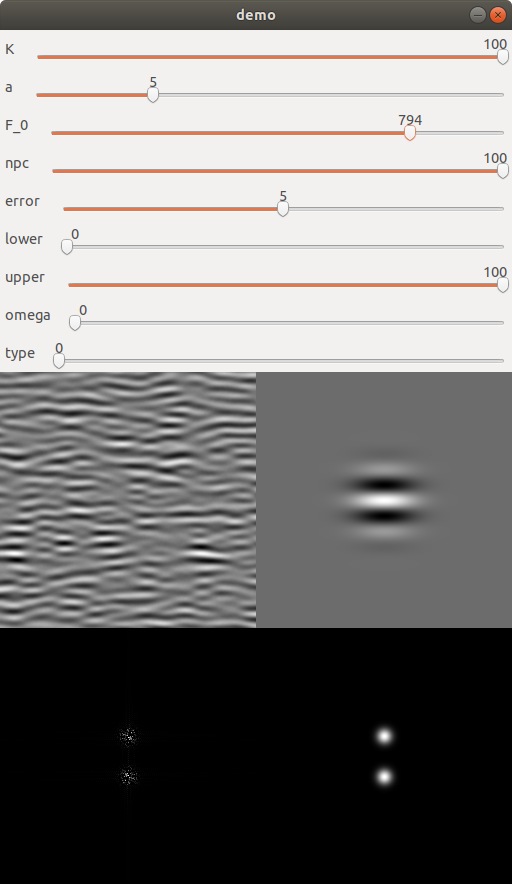
\includegraphics[width=0.3\textwidth]{ani.png}
    \caption{anisotropic noise}
  \end{figure}

  \begin{figure}[!hbt]
    \centering
    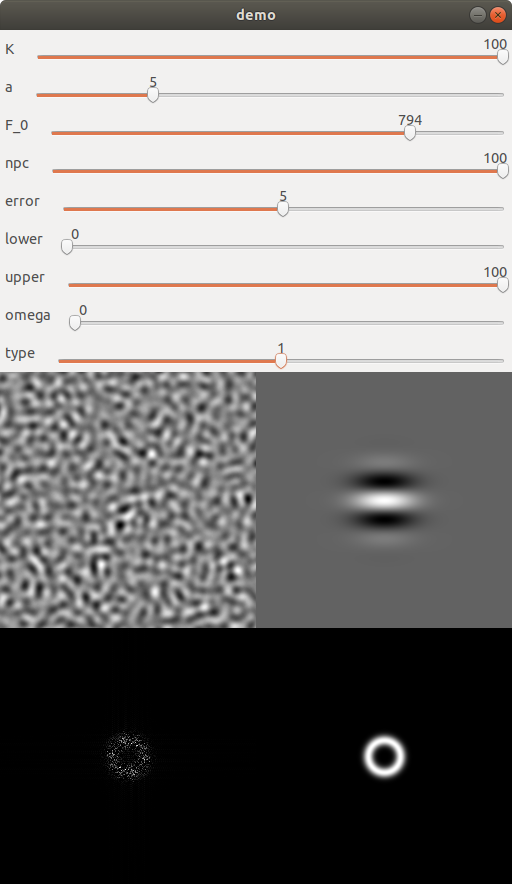
\includegraphics[width=0.3\textwidth]{iso.png}
    \caption{isotropic noise with anisotropic kernel}
  \end{figure}

  \begin{figure}[!hbt]
    \centering
    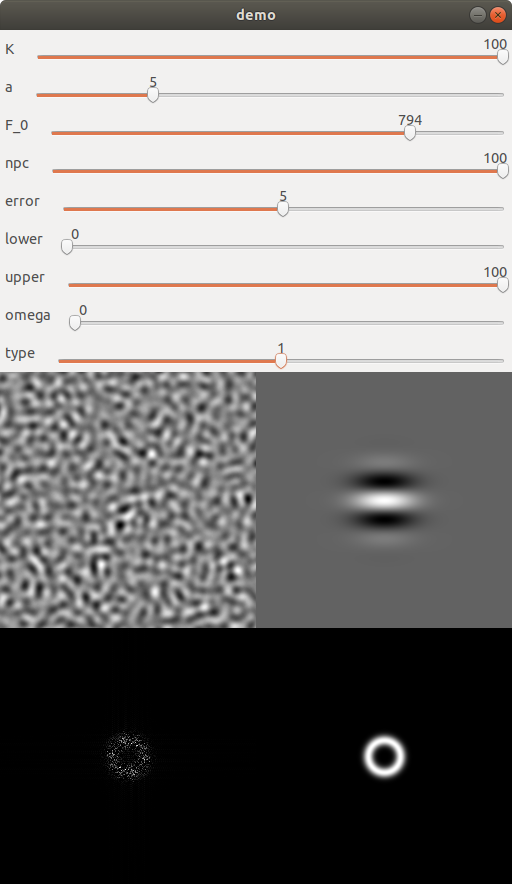
\includegraphics[width=0.3\textwidth]{iso.png}
    \caption{isotropic noise with isotropic kernel}
  \end{figure}

  \begin{figure}[!hbt]
    \centering
    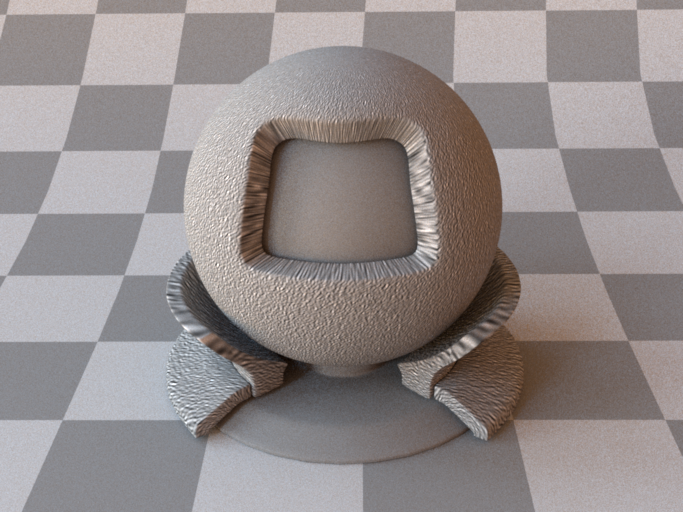
\includegraphics[width=0.3\textwidth]{ren1.png}
    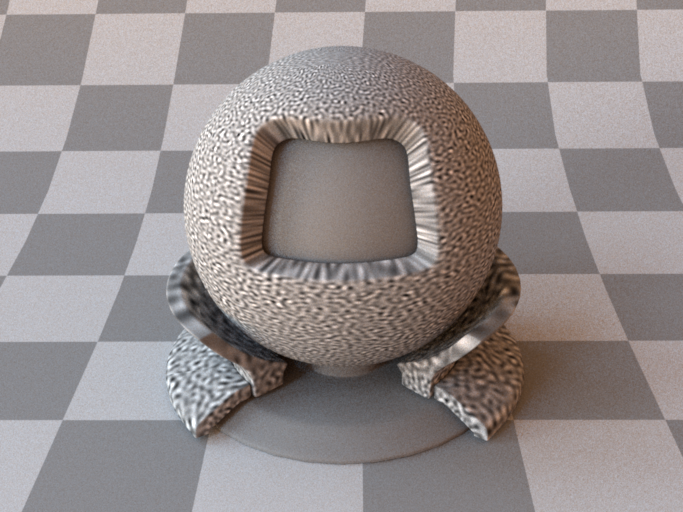
\includegraphics[width=0.3\textwidth]{ren2.png}
    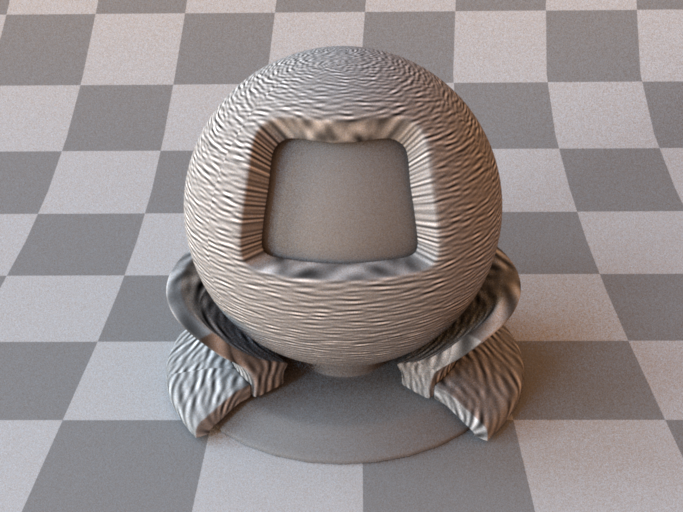
\includegraphics[width=0.3\textwidth]{ren3.png}
    \caption{Using the noise as texture}
  \end{figure}

  

% Now we need a bibliography:
\bibliographystyle{plain}  
\bibliography{ref}

% Your document ends here!
\end{document}